% This is LLNCS.DEM the demonstration file of
% the LaTeX macro package from Springer-Verlag
% for Lecture Notes in Computer Science,
% version 2.4 for LaTeX2e as of 16. April 2010
%
\documentclass{llncs}
%
\usepackage{amsmath}
\usepackage{amssymb}
\usepackage{tikz}
\usepackage[linesnumbered,ruled]{algorithm2e}

\newcounter{instr}
\newcommand{\ninstr}{\refstepcounter{instr}\theinstr.}

\begin{document}

\title{Species delimitation}

\titlerunning{Species delimitation}

\author{Tom\'{a}\v{s} Flouri\inst{1} \and Paschalia Kapli\inst{1} \and Sarah Lutteropp\inst{1}}
\authorrunning{Tom\'{a}\v{s} Flouri et al.} % abbreviated author list
\institute{Heidelberg Institute of Theoretical Studies}

\maketitle

\begin{abstract}
An explanation of the single-lambda and multiple-lambda heuristic for PTP.\@
\end{abstract}

\section{Related Work}

Like in the algorithm from Gulek et al.\cite{Gulek:2010:DPA:1838770.1839019} for the tree-like weighted set packing problem, we try to build up a solution for the whole tree by combining the solutions for its children subtrees.

\section{Task Description}

Given a rooted fully binary tree with non-negative edge weight function $w$, we want to partition its leaves into disjoint sets (called species). The \emph{most recent common ancestors} (MRCA) of those species induce subtrees with edge sets $E_1, \ldots, E_{k}$. Every edge that is not assigned to one of those subtrees is then put into the set of speciation edges, $E_{k+1}$.

Given a set of edges $E$, we define its log-likelihood $logl(E)$ as
$$logl(E) := |E| * (\log{|E|} - 1 - \log{\sum_{e \in E} w(e)})$$

\paragraph{Multiple Lambda Score}

We want to find a delimitation that maximizes the following sum of loglikelihoods (in the following referred to as \emph{score}):

$$\sum_{i=1}^{k+1}{logl(E_i)}$$

\paragraph{Single Lambda Score}

We want to find a delimitation that maximizes the following sum of loglikelihoods (in the following referred to as \emph{score}, too):

$$logl(\cup_{i=1}^k{E_i}) + logl(E_{k+1})$$

\section{The Heuristic}
We follow a bottom-up dynamic programming approach, always trying to extend a good solution for the children subtrees in order to obtain a good solution for the currently observed tree.

\subsection{Currently observed tree}

For each node $v$, the \emph{currently observed tree} (COT) consists of the subtree rooted at $v$, $S(v)$, and the set of edges where we already know that they have to be speciation edges in the case that $S(v)$ contains new species (see Fig.~\ref{fig:currently_observed_tree}). Our aim is to find a delimitation that yields to a high score for the COT.\@ This means that the score computation ignores all edges that are not in the COT since we do not know their assignment.

\begin{figure}[h!]
	\centering
	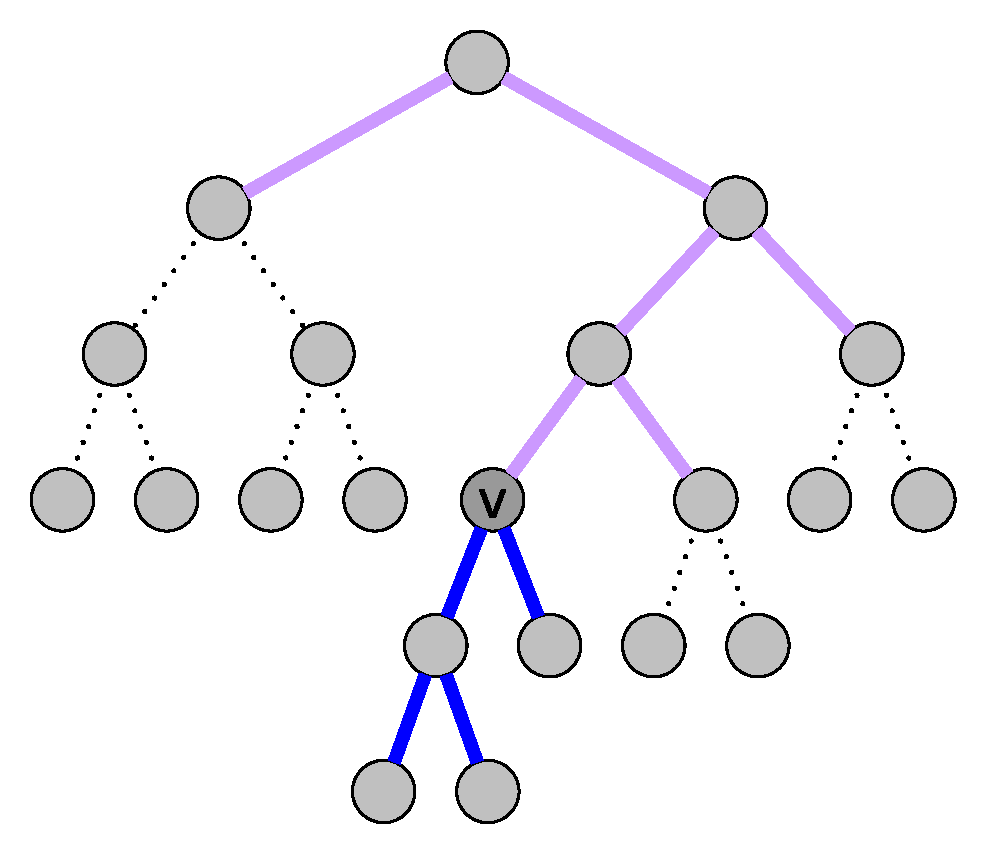
\includegraphics[scale=0.4]{images/currently_observed_tree.pdf}
	\caption{The COT of a node $v$. The edges belonging to $S(v)$ are drawn in thick blue lines and the known speciation edges are drawn in thick purple lines. Edges that do not belong to the COT of $v$ are drawn in dotted lines.}
	\label{fig:currently_observed_tree}
\end{figure}

\subsection{Combination of solutions}

For every node $v$, we store an array that contains the best found score for $0, 1, 2, 3, \ldots, |S(v)|$ speciation edges and the delimitation (i.e., the set of MRCAs) that led to it. A node $v$ can either be a coalescent event or a speciation event.

\paragraph{Coalescent event}
If $v$ is a coalescent event (i.e., the MRCA of a species), we have $0$ speciation edges in $S(v)$. For this case, we compute the score of all edges in $S(v)$ being coalescent edges and the known speciation edges in the COT of $v$ being speciation edges and store it in $v$. Since we do not need to look at the solutions for the children of $v$ in this case, we can do this step already in the initialization.

\paragraph{Speciation event}
In order to find a solution for a subtree $S(v)$ and $k \geq 1$ speciation edges, we combine the best found solution for $i$ speciation edges from the left child of $v$ with the best found solution for $j$ speciation edges for the right child of $v$ for all choices of $i$ and $j$ where $i+j+2$ sums up to $k$ (see Fig.~\ref{fig:combining}). We compute the score of the combined delimitations using either the single-lambda or multiple-lambda approach. Then we store the delimitation that yields to the highest score for $k$ speciation edges inside $v$.

\begin{figure}[h!]
\centering
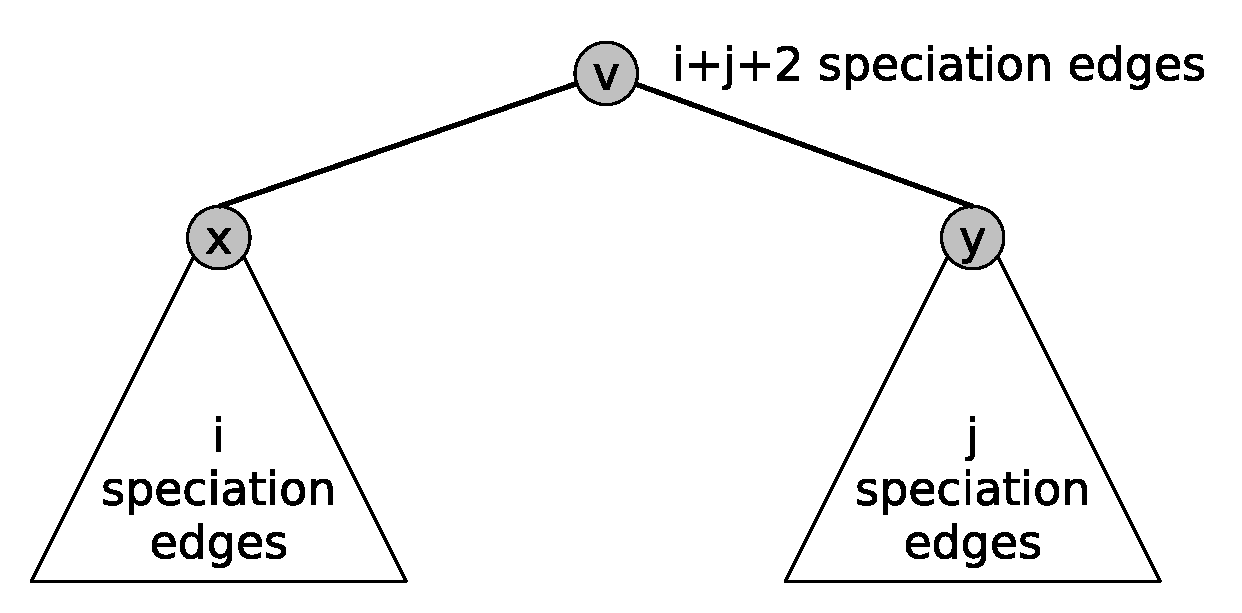
\includegraphics[scale=0.3]{images/speciation_events.pdf}
\caption{Combining the best found solutions for the subtrees}
\label{fig:combining}
\end{figure}

\subsection{Handling of too small Edges}

We allow the user to specify a minimum branch length $min\_br \geq 0$ such that all all edges with length \textbf{less or equal} $min\_br$ will be ignored in the loglikelihood score computation. Ignoring an edge means that we do not count it towards the number of edges and we do not add its length to the sum of edge weights.

\subsection{Final Result}
We obtain the final result by choosing the delimitation that led to the highest score for the root of the tree.

\subsection{Pseudocode}
\begin{algorithm}
\SetKwInOut{Input}{Input}
\SetKwInOut{Output}{Output}

\Input{A fully binary rooted tree $T$ with non-negative edge weights $w$, a minimum branch length $min\_br$}
\Output{A delimitation with maximal score}

\underline{function delimit $(T, min\_br)$}\

initialization(root($T$)$, min\_br$)\;
combineSolutions(root($T$))\;

delimitations = root($T$).delimitations\;

bestScore = scores[0]\;
bestIndex = 0\;

\For{$i = 1, \ldots, $ number of edges in $T$}{
	\If{delimitations[i].isValid}{
		\If{delimitations[i].score $>$ bestScore}{
			bestScore = delimitations[i].score\;
			bestIndex = i\;
		}
	}
}

\Return{delimitations[bestIndex]}

\caption{The heuristic for the PTP species delimitation problem, Main Loop}

\end{algorithm}


\begin{algorithm}
\SetKwInOut{Input}{Input}
\SetKwInOut{Output}{Output}

\Input{A vertex $v$, a minimum branch length $min\_br$}

\underline{function initialization $(v, min\_br)$}\

$v$.knownSpeciationEdges = $\emptyset$\;

\If{$v$.hasParent()} {
	$v$.knownSpeciationEdges.addAll(parent($v$).knownSpeciationEdges)\;
	$v$.knownSpeciationEdges.add($(\text{parent}(v),v)$)\;
	\If{$v$ == parent($v$).leftChild}{
		$v$.knownSpeciationEdges.add($(\text{parent}(v), \text{parent}(v).\text{rightChild})$)\;
	}
	\Else{
		$v$.knownSpeciationEdges.add($(\text{parent}(v), \text{parent}(v).\text{leftChild})$)\;
	}
}

\For{$i = 1, \ldots, |S(v)|$} {
	$v$.delimitations[i].isValid = False\;
	$v$.delimitations[i].score = $- \infty$\;
}

$v$.coalescentValue = computeLoglikelihoodScore(edges of $S(v)$, $min\_br$)\;

$v$.delimitations[0].score = $v$.coalescentValue + computeLoglikelihoodScore($v$.knownSpeciationEdges, $min\_br$)\;
$v$.delimitations[0].mostRecentCommonAncestors = $\{v\}$\;
$v$.delimitations[0].isValid = True\;

\If{$v$.hasLeftChild()} {
	initialization($v$.leftChild, $min\_br$)\;
}
\If{$v$.hasRightChild()} {
	initialization($v$.leftRight, $min\_br$)\;
}
\Return{}

\caption{The heuristic for the PTP species delimitation problem, Initialization}

\end{algorithm}

\begin{algorithm}
\SetKwInOut{Input}{Input}
\SetKwInOut{Output}{Output}

\Input{A set of edges $E$ non-negative edge weights $w$, a minimum branch length $min\_br$}
\Output{The loglikelihood score of $E$ with edges $\leq min\_br$ ignored}

\underline{function computeLoglikelihoodScore $(E, min\_br)$}\

sum = 0\;
num = 0\;
score = 0\;

\For{$e \in E$}{
	\If{$w(e) > min\_br$}{
		num++\;
		sum += $w(e)$\;
	}
}

\If {num $> 0$ \textbf{ and } sum $> 0$} {
	score = num * (log(num) - 1 - log(sum))\;
}

\Return{score}

\caption{The heuristic for the PTP species delimitation problem, Score computation}

\end{algorithm}



\begin{algorithm}
\SetKwInOut{Input}{Input}
\SetKwInOut{Output}{Output}

\Input{A vertex $v$, a minimum branch length $min\_br$}

\underline{function combineSolutions $(v, min\_br)$}\

\If{$v$.hasLeftChild()} {
	combineSolutions($v$.leftChild, $min\_br$)\;
}
\If{$v$.hasRightChild()} {
	combineSolutions($v$.leftRight, $min\_br$)\;
}

\If{$v$.hasLeftChild() \textbf{and} $v$.hasRightChild()} {
	\For{$k = 0, \ldots, |S(v)|$} {
		\For{$i = 0, \ldots, k - 2$} {
			\For{$j = 0, \ldots, k - 2 - i$} {
				\If{$v$.leftChild.delimitations[$i$].isValid \textbf{and} $v$.rightChild.delimitations[$j$].isValid}{
					currentMRCAList = $v$.leftChild.delimitations[i].mostRecentCommonAncestors $\cup$ $v$.rightChild.delimitations[j].mostRecentCommonAncestors\;
					currentlyObservedTreeEdges = $v$.knownSpeciationEdges $\cup$ edges of $S(v)$\;
					\If{multipleLambda} {
						currentCoalescentScore = $\sum_{m \in \text{currentMRCAList}} {\text{computeLoglikelihoodScore(edges of $S(m)$, min\_br)}}$
					}
					\Else {
						currentCoalescentScore = computeLoglikelihoodScore($\bigcup_{m \in \text{currentMRCAList}} {\text{edges of } S(m)}, min\_br)$\;
					}
					currentSpeciationScore = computeLoglikelihoodScore(currentlyObservedTreeEdges $\backslash \bigcup_{m \in \text{currentMRCAList}} {\text{edges of } S(m)}, min\_br)$\;
					currentScore = currentCoalescentScore + currentSpeciationScore\;
					\If{currentScore $>$ $v$.delimitations[k].score} {
						$v$.delimitations[k].mostRecentCommonAncestors = currentMRCAList\;
						$v$.delimitations[k].score = currentScore\;
						$v$.delimitations[k].valid = True\;
					}
				}
			}
		}
	}
}

\Return{}

\caption{The heuristic for the PTP species delimitation problem, Heuristic steps}

\end{algorithm}

\bibliographystyle{splncs03}
\bibliography{delimit}
\end{document}
